\ifx\wholebook\relax \else
% ------------------------ 

\documentclass{article}
%------------------- Other types of document example ------------------------
%
%\documentclass[twocolumn]{IEEEtran-new}
%\documentclass[12pt,twoside,draft]{IEEEtran}
%\documentstyle[9pt,twocolumn,technote,twoside]{IEEEtran}
%
%-----------------------------------------------------------------------------
%%
% loading packages
%
\newif\ifpdf
\ifx\pdfoutput\undefined % We're not running pdftex
  \pdffalse
\else
  \pdftrue
\fi
%
%
\ifpdf
  \RequirePackage[pdftex,%
            CJKbookmarks,%
       bookmarksnumbered,%
              colorlinks,%
          linkcolor=blue,%
              hyperindex,%
        plainpages=false,%
       pdfstartview=FitH]{hyperref}
\else
  \RequirePackage[dvipdfm,%
             CJKbookmarks,%
        bookmarksnumbered,%
               colorlinks,%
           linkcolor=blue,%
               hyperindex,%
         plainpages=false,%
        pdfstartview=FitH]{hyperref}
  \AtBeginDvi{\special{pdf:tounicode GBK-EUC-UCS2}} % GBK -> Unicode
\fi
\usepackage{hyperref}

% other packages
%-----------------------------------------------------------------------------
\usepackage{graphicx, color}
\usepackage{CJK}
%
% for programming 
%
\usepackage{verbatim}
\usepackage{listings}


\lstdefinelanguage{Smalltalk}{
  morekeywords={self,super,true,false,nil,thisContext}, % This is overkill
  morestring=[d]',
  morecomment=[s]{"}{"},
  alsoletter={\#:},
  escapechar={!},
  literate=
    {BANG}{!}1
    {UNDERSCORE}{\_}1
    {\\st}{Smalltalk}9 % convenience -- in case \st occurs in code
    % {'}{{\textquotesingle}}1 % replaced by upquote=true in \lstset
    {_}{{$\leftarrow$}}1
    {>>>}{{\sep}}1
    {^}{{$\uparrow$}}1
    {~}{{$\sim$}}1
    {-}{{\sf -\hspace{-0.13em}-}}1  % the goal is to make - the same width as +
    %{+}{\raisebox{0.08ex}{+}}1		% and to raise + off the baseline to match -
    {-->}{{\quad$\longrightarrow$\quad}}3
	, % Don't forget the comma at the end!
  tabsize=2
}[keywords,comments,strings]

\lstloadlanguages{C++, Lisp, Haskell, Python, Smalltalk}

% ======================================================================

\def\BibTeX{{\rm B\kern-.05em{\sc i\kern-.025em b}\kern-.08em
    T\kern-.1667em\lower.7ex\hbox{E}\kern-.125emX}}

\newtheorem{theorem}{Theorem}

%
% mathematics
%
\newcommand{\be}{\begin{equation}}
\newcommand{\ee}{\end{equation}}
\newcommand{\bmat}[1]{\left( \begin{array}{#1} }
\newcommand{\emat}{\end{array} \right) }
\newcommand{\VEC}[1]{\mbox{\boldmath $#1$}}

% numbered equation array
\newcommand{\bea}{\begin{eqnarray}}
\newcommand{\eea}{\end{eqnarray}}

% equation array not numbered
\newcommand{\bean}{\begin{eqnarray*}}
\newcommand{\eean}{\end{eqnarray*}}

\RequirePackage{CJK,CJKnumb,CJKulem,CJKpunct}
% we use CJK as default environment
\AtBeginDocument{\begin{CJK*}{GBK}{song}\CJKtilde\CJKindent\CJKcaption{GB}}
\AtEndDocument{\clearpage\end{CJK*}}

%
% loading packages
%

\RequirePackage{ifpdf}

%
%
\ifpdf
  \RequirePackage[pdftex,%
       bookmarksnumbered,%
              colorlinks,%
          linkcolor=blue,%
              hyperindex,%
        plainpages=false,%
       pdfstartview=FitH]{hyperref}
\else
  \RequirePackage[dvipdfm,%
        bookmarksnumbered,%
               colorlinks,%
           linkcolor=blue,%
               hyperindex,%
         plainpages=false,%
        pdfstartview=FitH]{hyperref}
\fi
\usepackage{hyperref}

% other packages
%--------------------------------------------------------------------------
\usepackage{graphicx, color}
\usepackage{subfig}

\usepackage{amsmath, amsthm, amssymb} % for math
\usepackage{exercise} % for exercise

%
% for programming 
%
\usepackage{verbatim}
\usepackage{listings}
%\usepackage{algorithmic} %old version; we can use algorithmicx instead
\usepackage{algorithm} 
\usepackage[noend]{algpseudocode} %for pseudo code, include algorithmicsx automatically
\usepackage{makeidx} % for index support


\lstdefinelanguage{Smalltalk}{
  morekeywords={self,super,true,false,nil,thisContext}, % This is overkill
  morestring=[d]',
  morecomment=[s]{"}{"},
  alsoletter={\#:},
  escapechar={!},
  literate=
    {BANG}{!}1
    {UNDERSCORE}{\_}1
    {\\st}{Smalltalk}9 % convenience -- in case \st occurs in code
    % {'}{{\textquotesingle}}1 % replaced by upquote=true in \lstset
    {_}{{$\leftarrow$}}1
    {>>>}{{\sep}}1
    {^}{{$\uparrow$}}1
    {~}{{$\sim$}}1
    {-}{{\sf -\hspace{-0.13em}-}}1  % the goal is to make - the same width as +
    %{+}{\raisebox{0.08ex}{+}}1		% and to raise + off the baseline to match -
    {-->}{{\quad$\longrightarrow$\quad}}3
	, % Don't forget the comma at the end!
  tabsize=2
}[keywords,comments,strings]

\lstloadlanguages{C++, Lisp, Haskell, Python, Smalltalk}

% ======================================================================

\def\BibTeX{{\rm B\kern-.05em{\sc i\kern-.025em b}\kern-.08em
    T\kern-.1667em\lower.7ex\hbox{E}\kern-.125emX}}

%
% mathematics
%
\newcommand{\be}{\begin{equation}}
\newcommand{\ee}{\end{equation}}
\newcommand{\bmat}[1]{\left( \begin{array}{#1} }
\newcommand{\emat}{\end{array} \right) }
\newcommand{\VEC}[1]{\mbox{\boldmath $#1$}}

% numbered equation array
\newcommand{\bea}{\begin{eqnarray}}
\newcommand{\eea}{\end{eqnarray}}

% equation array not numbered
\newcommand{\bean}{\begin{eqnarray*}}
\newcommand{\eean}{\end{eqnarray*}}

\newtheorem{theorem}{Theorem}[section]
\newtheorem{lemma}[theorem]{Lemma}
\newtheorem{proposition}[theorem]{Proposition}
\newtheorem{corollary}[theorem]{Corollary}


\setcounter{page}{1}

\begin{document}

\fi
%--------------------------

% ================================================================
%                 COVER PAGE
% ================================================================

\title{Suffix Tree with Functional and imperative implementation}

\author{Liu~Xinyu
\thanks{{\bfseries Liu Xinyu } \newline
  Email: liuxinyu95@gmail.com \newline}
%  Tel:   +86-1305-196-8666 \newline}
  }

\markboth{Suffix Tree}{Imperative and Functional}

\maketitle

\ifx\wholebook\relax
\chapter{Suffix Tree with Functional and imperative implementation}

\section{abstract}
\else
\begin{abstract}
\fi
Suffix Tree is an important data structure. It is quite powerful in 
string and DNA informaiton manipulations. Suffix Tree is introduced in 1973.
The latest online construction algorithm was found in 1995. This post 
collects some existing result of suffix tree, including the construction
algorithms as well as some typical applications. Some imperative and functional
implementation are given. There are multiple programming languages used, 
including C++, Haskell, Python and Scheme/Lisp.

There may be mistakes in the post, please feel free to point out.

This post is generated by \LaTeXe, and provided with GNU FDL(GNU Free Documentation License).
Please refer to http://www.gnu.org/copyleft/fdl.html for detail.

\ifx\wholebook\relax\else
\end{abstract}
\fi

\vspace{3cm}
{\bfseries Keywords:} Suffix Tree

%{\bfseries Corresponding Author:} Liu Xinyu

\maketitle

% ================================================================
%                 Introduction
% ================================================================
\section{Introduction}
\label{introduction}

Suffix Tree is a special Patricia. There is no such a chapter
in CLSR book. To introduce suffix tree together with Trie and Patricia
will be a bit easy to understand. 

As a data structure, Suffix tree allows for paticulary fast implementation
of many important string operations\cite{wiki-suffix-tree}. And it is 
also widely used in bio-information area such as DNA pattern 
matching\cite{ukkonen-presentation}.

The suffix tree for a string $S$ is a Patricia tree, with each edges are labeled
with some sub-string of $S$. Each suffix of $S$ corresponds to exactly one path
from root to a leaf. Figure \ref{fig:stree-banana} shows the suffix tree for
an English word `banana'.

\begin{figure}[htbp]
       \begin{center}
	\includegraphics[scale=0.5]{img/stree-banana.ps}
        \caption{The suffix tree for `banana'} \label{fig:stree-banana}
       \end{center}
\end{figure}

Note that all suffixes, 'banana', 'anana', 'nana', 'ana', 'na', 'a', '' can 
be looked up in the above tree. Among them the first 3 suffixes are explicitly
shown; others are implicitly represented. The reason for why 'ana, 'na', 'a', 
and '' are not shown explicitly is because they are prefixes of some edges.
In order to make all suffixes shown explicitly, we can append a special pad 
terminal symbal, which is not seen to the string. Such terminator is typically
denoted as '\$'. With this method, no suffix will be a prefix of the others.
In this post, we won't use terminal symbol for most cases.

It's very interesting that compare to the simple suffix tree for 'banana', the
suffix tree for 'bananas' is quite different as shown in figure \ref{fig:stree-bananas}.

\begin{figure}[htbp]
       \begin{center}
	\includegraphics[scale=0.5]{img/stree-bananas.ps}
        \caption{The suffix tree for `bananas'} \label{fig:stree-bananas}
       \end{center}
\end{figure}

In this post, I'll first introduce about suffix Trie, and give the trivial method
about how to construct suffix Trie and tree. Trivial methods utilize the insertion
algorithm for normal Trie and patricia. They need much of computation and spaces.
Then, I'll explain about the online construction for suffix Trie by using suffix link
concept. After that, I'll show Ukkonen's method, which is a linear time online 
construction algorithm. For both suffix Trie and suffix tree, functional approach
is provided as well as the imperative one. In the last section, I'll list some
typical string manipulation problems and show how to solve them with suffix tree.

This article provides example implementation in C, C++, Haskell, Python, and 
Scheme/Lisp languages. 

All source code can be downloaded in appendix \ref{appendix}, please 
refer to appendix for detailed information about build and run.

% ================================================================
%                 Suffix Trie
% ================================================================
\section{Suffix Trie}
\label{suffix-trie}

Just likes the relationship between Trie and Patricia, Suffix Trie has much simpler
structure than suffix tree. Figure \ref{fig:strie-banana} shows the suffix Trie of
'banana'.

\begin{figure}[htbp]
       \begin{center}
	\includegraphics[scale=0.5]{img/strie-banana.ps}
        \caption{Suffix Trie of 'banana'} \label{fig:strie-banana}
       \end{center}
\end{figure}

Compare with figure \ref{fig:stree-banana}, the difference is that, instead of representing
a word for each edge, one edge in suffix Trie only represents one character. Thus
suffix Trie need more spaces. If we pack all nodes which has only one child, the suffix
Trie can be turned into a suffix tree.

Suffix Trie can be a good start point for explaining the suffix tree construction algorithm.

%=========================================================================
%       Trivial construction of Suffix Trie and Suffix Tree
%=========================================================================
\section{Trivial construction methods of Suffix Tree}
\label{trivial-cons}

By repeatly applying the insertion algorithms\cite{lxy-trie} for Trie and Patricia
on each suffixes of a word, Suffix Trie and tree can be built in a trivial way.

Below algorithm illustrates this approach for suffix tree.

\begin{algorithmic}
\STATE $TRIVIAL-SUFFIX-TREE(S)$
  \STATE $T \leftarrow NIL$
  \FOR{$i$ from $1$ to $LENGTH(S)$}
    \STATE $T \leftarrow PATRICIA-INSERT(T, RIGHT(S, i))$
  \ENDFOR
  \RETURN $T$
\end{algorithmic}

Where function $RIGHT(S, i)$ will extract substring of S from left to right most.
Similar functional algorithm can also be provided in this way.

\begin{algorithmic}
\STATE $TRIVIAL-SUFFIX-TREE'(S)$
  \RETURN $FOLD-LEFT(PATRICIA-INSERT, NIL, TAILS(S))$
\end{algorithmic}

Function TAILS() returns a list of all suffixes for string S. In Haskell, Module 
Data.List provides this function already. In Scheme/Lisp, it can be implemented as below.

\lstset{language=lisp}
\begin{lstlisting}
(define (tails s)
  (if (string-null? s)
      '("")
      (cons s (tails (string-tail s 1)))))
\end{lstlisting}

The trivial suffix Trie/tree construction method takes $O(n^2)$ time, where $n$ is the 
length of the word. Altough the string manipulation can be very fast by using suffix
tree, slow construction will be the bottleneck of the whole process.

% ================================================================
%               Online construction of Suffix Trie
% ================================================================
\section{Online construction of suffix trie}

Analysis of construction for suffix Trie can be a good start point in finding
the linear time suffix tree construction algorithm. In Ukkonen's paper\cite{ukkonen95}, 
finite-state automation, transition function and suffix function are used to 
build the mathematical model for suffix Trie/tree. 

In order to make it easy for understanding, let's explain the above concept with
the elements of Trie data structure.

With a set of alphabetic, a string with length $n$ can be defined as $S=s_1s_2...s_n$.
And we define $S[i]=s_1s_2...s_i$, which contains the first $i$ characters.

In a suffix Trie, each node represents a suffix string. for example in figure 
\ref{fig:strie-cacao}, node X represents suffix 'a', by adding a character 'c',
node X transfers to node Y which represents suffix 'ac'. We say node X and edge labelled 'c'
transfers to node Y. This relation ship can be denoted in psuedo code as below.

\begin{figure}[htbp]
       \begin{center}
	\includegraphics[scale=0.5]{img/strie-cacao.ps}
        \caption{node $X \leftarrow 'a'$, node $Y \leftarrow 'ac'$, $X$ transfer to $Y$ with character 'c'}
        \label{fig:strie-cacao}
       \end{center}
\end{figure}

\begin{algorithmic}
\STATE $Y \leftarrow CHILDREN(X)[c]$
\end{algorithmic}

It's equal to the following C++ and Python code.

Next: suffix link

\lstset{language=python}
\begin{lstlisting}
y = x.children[c]
\end{lstlisting}


\subsubsection*{Insertion of integer Trie in Scheme/Lisp}

Insertion program implemented with Scheme/Lisp is quite similar, since
Scheme has a complex numeric system, it will use fraction instead of
round to integer, we minus the key by 1 before divide it with 2.

\lstset{language=lisp}
\begin{lstlisting}
;; Insertion
;;   if user insert an existed value, just overwrite the old value
;;   usage: (insert t k x) t: trie, k: key, x: value
(define (insert t k x)
  (if (= k 0)
      (make-int-trie (left t) x (right t))
      (if (even? k)
	  (make-int-trie (insert (left t) (/ k 2) x) (value t) (right t))
	  (make-int-trie (left t) (value t) (insert (right t) (/ (- k 1) 2) x)))))
\end{lstlisting}

In order to make creation of Trie from a list of key-value pairs easy,
here is a helper function.

\begin{lstlisting}
(define (list->trie lst) ;;lst is list of pairs
  (define (insert-pair t p)
    (insert t (car p) (cadr p)))
  (fold-left insert-pair '() lst))
\end{lstlisting}

In order to convert the Trie to a readable string, a converter
function is given as the following.

\begin{lstlisting}
(define (trie->string trie)
  (define (value->string x)
    (cond ((null? x) ".")
	  ((number? x) (number->string x))
	  ((string? x) x)
	  (else "unknown value")))
  (define (trie->str t k m)
    (if (null? t)
	"."
	(string-append "(" (trie->str (left t) k (* m 2)) " "
		       (number->string k) (value->string (value t)) " "
		       (trie->str (right t) (+ m k) (* m 2)) ")")))
  (trie->str trie 0 1))
\end{lstlisting}

To verify the program, we can test it with a easy test case.

\begin{lstlisting}
(define (test-int-trie)
  (define t (list->trie (list '(1 "a") '(4 "b") '(5 "c") '(9 "d"))))
  (display (trie->string t)) (newline))
\end{lstlisting}

Evaluate this test function will generate below output.

\begin{lstlisting}
(test-int-trie)
(((. 0. (. 4b .)) 0. .) 0. (((. 1. (. 9d .)) 1. (. 5c .)) 1a .))
\end{lstlisting}

Which is identical to the Haskell output.

% ================================================================
%               Online construction of suffix tree
% ================================================================
\subsection{Online construction of suffix tree} 

\subsubsection{Iterative looking up algorithm}

To look up a key in a little-endian integer binary trie. We take each
bit of the key from left (LSB), and go left or right according to if
the bit is 0, until we consumes all bits. this algorithm can be described
as below pseudo code.

\begin{algorithmic}
\STATE $INT-TRIE-LOOKUP(T, x)$
  \WHILE{$x \neq 0$ and $T \neq NIL$}
    \IF{$EVEN(x) = TRUE$}
      \STATE $T \leftarrow LEFT(T)$
    \ELSE
      \STATE $T \leftarrow RIGHT(T)$
    \ENDIF
    \STATE $x \leftarrow x/2$
  \ENDWHILE
  \IF{$T \neq NIL$} \RETURN $DATA(T)$
  \ELSE \RETURN $NIL$ \ENDIF
\end{algorithmic}

\subsubsection*{Look up implemented in C++}
In C++, we can test the LSB by using bit-wise operation. The following code
snippet searches a key in an integer Trie. If the target node is found, the
value of that node is returned, else it will return the default value of the
value type\footnote{One good alternative is to raise exception if not found}.
\lstset{language=C++}
\begin{lstlisting}
template<class T>
T lookup(IntTrie<T>* t, int key){
  while(key && t){
    if( (key & 0x1) == 0)
      t = t->left;
    else
      t = t->right;
    key>>=1;
  }
  if(t)
    return t->value;
  else
    return T();
}
\end{lstlisting}

To verify this program, some simple test cases are provided.

\begin{lstlisting}
std::cout<<"\nlook up 4: "<<lookup(tc, 4)
         <<"\nlook up 9: "<<lookup(tc, 9)
         <<"\nlook up 0: "<<lookup(tc, 0);
\end{lstlisting}

Where 'tc' is the Trie we created in insertion section. the output is like below.
\begin{verbatim}
look up 4: b
look up 9: d
look up 0: 
\end{verbatim}

\subsubsection*{Look up implemented in Python}
By translating the pseudo code algorithm, we can easily get a python 
implementation.

\lstset{language=Python}
\begin{lstlisting}
def lookup(t, key):
    while key != 0 and (t is not None):
        if key & 1 == 0:
            t = t.left
        else:
            t = t.right
        key = key>>1
    if t is not None:
        return t.value
    else:
        return None
\end{lstlisting}

In this implementation, instead of using even-odd property, bit-wise
manipulation is used to test if a bit is 0 or 1.

Here is the smoke test of the lookup function.

\begin{lstlisting}
class IntTrieTest:
    #...
    def test_lookup(self):
        t = map_to_trie({4:'y', 1:'x', 5:'z'})
        print "look up 4: ", lookup(t, 4)
        print "look up 5: ", lookup(t, 5)
        print "look up 0: ", lookup(t, 0)
\end{lstlisting}

The output of the test cases is as below.

\begin{verbatim}
look up 4:  y
look up 5:  z
look up 0:  None
\end{verbatim}

\subsubsection{Recursive looking up algorithm}

Looking up in integer Trie can also be implemented in recursive manner.
We take the LSB of the key to be found, if it is 0, we recursively look
it up in left child, else in right child.

\begin{algorithmic}
\STATE $INT-TRIE-LOOKUP'(T, x)$
  \IF{$T = NIL$}
    \RETURN $NIL$
  \ELSIF{$x = 0$}
    \RETURN $VALUE(T)$
  \ELSIF{$EVEN(x)$}
    \RETURN $INT-TRIE-LOOKUP'(LEFT(T), x/2)$
  \ELSE
    \RETURN $INT-TRIE-LOOKUP'(RIGHT(T), x/2)$
  \ENDIF
\end{algorithmic}

\subsubsection*{Look up implemented in Haskell}
In Haskell, we can use pattern matching to realize the above long if-then-else statements.
The program is as the following.

\lstset{language=Haskell}
\begin{lstlisting}
search :: IntTrie a -> Key -> Maybe a
search Empty k = Nothing
search t 0 = value t
search t k = if even k then search (left t) (k `div` 2)
             else search (right t) (k `div` 2)
\end{lstlisting}

If trie is empty, we simply returns nothing; if key is zero we return the 
value of current node; in other case we recursively search either left
child or right child according to the LSB is 0 or not.

To test this program, we can write a smoke test case as following.

\begin{lstlisting}
testIntTrie = "t=" ++ (toString t) ++ 
              "\nsearch t 4: " ++ (show $ search t 4) ++
              "\nsearch t 0: " ++ (show $ search t 0)
    where
      t = fromList [(1, 'a'), (4, 'b'), (5, 'c'), (9, 'd')]

main = do
  putStrLn testIntTrie
\end{lstlisting}

This program will output these result.

\begin{verbatim}
t=(((. 0 (. 4:'b' .)) 0 .) 0 (((. 1 (. 9:'d' .)) 1 (. 5:'c' .)) 1:'a' .))
search t 4: Just 'b'
search t 0: Nothing
\end{verbatim}

\subsubsection*{Look up implemented in Scheme/Lisp}

Scheme/Lisp implementation is quite similar. Note that we decrees key
by 1 before divide it with 2.

\lstset{language=lisp}
\begin{lstlisting}
(define (lookup t k)
  (if (null? t) '()
      (if (= k 0) (value t)
	  (if (even? k) 
	      (lookup (left t) (/ k 2))
	      (lookup (right t) (/ (- k 1) 2))))))
\end{lstlisting}

Test cases use the same Trie which is created in insertion section.

\begin{lstlisting}
(define (test-int-trie)
  (define t (list->trie (list '(1 "a") '(4 "b") '(5 "c") '(9 "d"))))
  (display (trie->string t)) (newline)
  (display "lookup 4: ") (display (lookup t 4)) (newline)
  (display "lookup 0: ") (display (lookup t 0)) (newline))
\end{lstlisting}

the result is as same as the one output by Haskell program.

\begin{lstlisting}
(test-int-trie)
(((. 0. (. 4b .)) 0. .) 0. (((. 1. (. 9d .)) 1. (. 5c .)) 1a .))
lookup 4: b
lookup 0: ()
\end{lstlisting}

% ================================================================
%               Suffix tree applications
% ================================================================

\section{Suffix tree applications}
Trie and Patricia are widely used in software industry. Integer based
Patricia tree is widely used in compiler. Some daily
used software has very interesting features can be realized with 
Trie and Patricia. In the following sections, I'll list some of them,
including, e-dictionary, word auto-completion, t9 input method etc.
The commercial implementation typically doesn't adopt Trie or Patricia
directly. However, Trie and Patricia can be shown as a kind of 
example realization.

\subsection{e-dictionary and word auto-completion}
Figure \ref{fig:e-dict} shows a screen shot of an English-Chinese dictionary.
In order to provide good user experience, when user input something, 
the dictionary will search its word library, and list all candidate words and
phrases similar to what user have entered.

%\begin{figure}[htbp]
%       \begin{center}
%	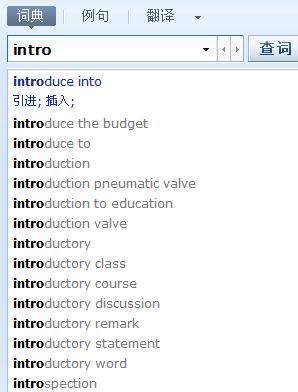
\includegraphics[scale=0.5]{img/ciba.eps}
%        \caption{e-dictionary. All candidates starting with what user input are listed.}
%        \label{fig:e-dict}
%       \end{center}
%\end{figure}

Typically such dictionary contains hundreds of thousands words, performs a whole
word search is expensive. Commercial software adopts complex approach, including
caching, indexing etc to speed up this process.

Similar with e-dictionary, figure \ref{fig:word-completion} shows a popular
Internet search engine, when user input something, it will provide a candidate
lists, with all items start with what user has entered. And these candidates
are shown in an order of popularity. The more people search for a word, the
upper position it will be shown in the list.

%\begin{figure}[htbp]
%       \begin{center}
%	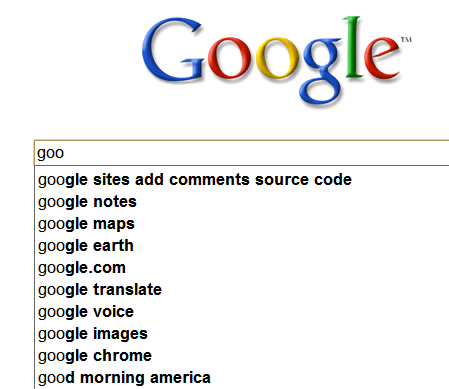
\includegraphics[scale=0.5]{img/adaptive-input.eps}
%        \caption{Search engine. All candidates key words starting with what user input are listed.}
%        \label{fig:word-completion}
%       \end{center}
%\end{figure}

In both case, we say the software provide a kind of word auto-completion support. 
In some modern IDE, the editor can even helps user to auto-complete programmings. 

In this section, I'll show a very simple implementation of e-dictionary with Trie
and Patricia.
To simplify the problem, let us assume the dictionary only support English - English
information.

Typically, a dictionary contains a lot of key-value pairs, the keys are English
words or phrases, and the relative values are the meaning of the words.

We can store all words and their meanings to a Trie, the drawback for this 
approach is that it isn't space effective. We'll use Patricia as alternative
later on.

As an example, when user want to look up 'a', the dictionary does not only
return the meaning of then English word 'a', but also provide a list of 
candidate words, which are all start with 'a', including 'abandon', 'about',
'accent', 'adam', ... Of course all these words are stored in Trie.

If there are too many candidates, one solution is only display the top 10
words for the user, and if he like, he can browse more.

Below pseudo code reuse the looking up program in previous sections and
Expand all potential top N candidates.

\begin{algorithmic}
\STATE $TRIE-LOOK-UP-TOP-N(T, key, N)$
  \STATE $p \leftarrow TRIE-LOOK-UP'(T, key)$
  \RETURN $EXPAND-TOP-N(p, key, N)$
\end{algorithmic}

Note that we should modify the TRIE-LOOK-UP a bit, instead of return
the value of the node, TRIE-LOOK-UP' returns the node itself.

Another alternative is to use Patricia instead of Trie. It can save much
spaces.

\subsubsection{Iterative algorithm of search top N candidate in Patricia}

The algorithm is similar to the Patricia look up one, but when we found
a node which key start from the string we are looking for, we expand
all its children until we get N candidates.

\begin{algorithmic}
\STATE $PATRICIA-LOOK-UP-TOP-N(T, key, N)$
  \IF{$T = NIL$}
     \RETURN $NIL$ \ENDIF

  \STATE $prefix \leftarrow NIL$
  \REPEAT
    \STATE $match \leftarrow FALSE$
    \FOR{each $i$ in $CHILDREN(T)$}
      \IF{$key$ IS-PREFIX-OF $KEY(i)$}
        \RETURN $EXPAND-TOP-N(TREE(i), prefix, N)$
      \ENDIF
      \IF{$KEY(i)$ IS-PREFIX-OF $key$}
        \STATE $match \leftarrow TRUE$
        \STATE $key \leftarrow key$ subtract $KEY(i)$
        \STATE $T \leftarrow TREE(i)$
        \STATE $prefix \leftarrow prefix + KEY(i)$
        \STATE break
      \ENDIF
    \ENDFOR
  \UNTIL{$match = FALSE$}
  \RETURN $NIL$
\end{algorithmic}

\subsubsection*{An e-dictionary in Python}
In Python implementation, a function trie\_lookup is provided to perform
search all top N candidate started with a given string.

\lstset{language=Python}
\begin{lstlisting}
def trie_lookup(t, key, n):
    if t is None:
        return None

    p = t
    for c in key:
        if not c in p.children:
            return None
        p=p.children[c]
    return expand(key, p, n)

def expand(prefix, t, n):
    res = []
    q = [(prefix, t)]
    while len(res)<n and len(q)>0:
        (s, p) = q.pop(0)
        if p.value is not None:
            res.append((s, p.value))
        for k, tr in p.children.items():
            q.append((s+k, tr))
    return res
\end{lstlisting}

Compare with the Trie look up function, the first part of this program is almost
same. The difference part is after we successfully located the node
which matches the key, all sub trees are expanded from this node in a 
bread-first search manner, and the top n candidates are returned. 

This program can be verified by below simple test cases.

\begin{lstlisting}
class LookupTest:
    def __init__(self):
        dict = {"a":"the first letter of English", \
           "an":"...same dict as in Haskell example"}
        self.tt = trie.map_to_trie(dict)

    def run(self):
        self.test_trie_lookup()

    def test_trie_lookup(self):
        print "test lookup top 5"
        print "search a ", trie_lookup(self.tt, "a", 5)
        print "search ab ", trie_lookup(self.tt, "ab", 5)
\end{lstlisting}

The test will output the following result.

\begin{verbatim}
test lookup to 5
search a  [('a', 'the first letter of English'), ('an', "used instead of 'a' 
when the following word begins with a vowel sound"), ('adam', 'a character in 
the Bible who was the first man made by God'), ('about', 'on the subject of; 
connected with'), ('abandon', 'to leave a place, thing or person forever')]
search ab  [('about', 'on the subject of; connected with'), ('abandon', 'to 
leave a place, thing or person forever')]
\end{verbatim}

To save the spaces, we can also implement such a dictionary search by using
Patricia.

\begin{lstlisting}
def patricia_lookup(t, key, n):
    if t is None:
        return None
    prefix = ""
    while(True):
        match = False
        for k, tr in t.children.items():
            if string.find(k, key) == 0: #is prefix of
                return expand(prefix+k, tr, n)
            if string.find(key, k) ==0:
                match = True
                key = key[len(k):]
                t = tr
                prefix += k
                break
        if not match:
            return None
\end{lstlisting}

In this program, we called Python string class to test if a string x is
prefix of a string y. In case we locate a node with the key we are looking
up is either equal of as prefix of the this sub tree, we expand it till
we find n candidates. Function expand() can be reused here.

We can test this program with the very same test cases and the results are
identical to the previous one.

\subsubsection*{An e-dictionary in C++}

In C++ implementation, we overload the look up function by providing an
extra integer n to indicate we want to search top n candidates. the
result is a list of key-value pairs, 

\lstset{language=C++}
\begin{lstlisting}
//lookup top n candidate with prefix key in Trie
template<class K, class V>
std::list<std::pair<K, V> > lookup(Trie<K, V>* t, 
                                   typename Trie<K, V>::KeyType key, 
                                   unsigned int n)
{
  typedef std::list<std::pair<K, V> > Result;
  if(!t)
    return Result();

  Trie<K, V>* p(t);
  for(typename K::iterator it=key.begin(); it!=key.end(); ++it){
    if(p->children.find(*it) == p->children.end())
      return Result();
    p = p->children[*it];
  }
  return expand(key, p, n);
}
\end{lstlisting}

The program is almost same as the Trie looking up one, except it will
call expand function when it located the node with the key. Function
expand is as the following.

\begin{lstlisting}
template<class T>
std::list<std::pair<typename T::KeyType, typename T::ValueType> >
expand(typename T::KeyType prefix, T* t, unsigned int n)
{
  typedef typename T::KeyType KeyType;
  typedef typename T::ValueType ValueType;
  typedef std::list<std::pair<KeyType, ValueType> > Result;

  Result res;
  std::queue<std::pair<KeyType, T*> > q;
  q.push(std::make_pair(prefix, t));
  while(res.size()<n && (!q.empty())){
    std::pair<KeyType, T*> i = q.front();
    KeyType s = i.first;
    T* p = i.second;
    q.pop();
    if(p->value != ValueType()){
      res.push_back(std::make_pair(s, p->value));
    }
    for(typename T::Children::iterator it = p->children.begin();
        it!=p->children.end(); ++it)
      q.push(std::make_pair(s+it->first, it->second));
  }
  return res;
}
\end{lstlisting}

This function use a bread-first search approach to expand top N
candidates, it maintain a queue to store the node it is currently
dealing with. Each time the program picks a candidate node from the
queue, expands all its children and put them to the queue. the program
will terminate when the queue is empty or we have already found N
candidates. 

Function expand is generic we'll use it in later sections.

Then we can provide a helper function to convert the candidate
list to readable string. Note that this list is actually a list of pairs so we can
provide a generic function.

\begin{lstlisting}
//list of pairs to string
template<class Container>
std::string lop_to_str(Container coll){
  typedef typename Container::iterator Iterator;
  std::ostringstream s;
  s<<"[";
  for(Iterator it=coll.begin(); it!=coll.end(); ++it)
    s<<"("<<it->first<<", "<<it->second<<"), ";
  s<<"]";
  return s.str();
}
\end{lstlisting}

After that, we can test the program with some simple test cases.

\begin{lstlisting}
Trie<std::string, std::string>* t(0);
const char* dict[] = {
  "a", "the first letter of English", \
  "an", "used instead of 'a' when the following word begins with a vowel sound", \
  "another", "one more person or thing or an extra amount", \
  "abandon", "to leave a place, thing or person forever", \
  "about", "on the subject of; connected with", \
  "adam", "a character in the Bible who was the first man made by God", \
  "boy", "a male child or, more generally, a male of any age", \
  "body", "the whole physical structure that forms a person or animal", \
  "zoo", "an area in which animals, especially wild animals, are kept" \
         "so that people can go and look at them, or study them"};

const char** first=dict;
const char** last =dict + sizeof(dict)/sizeof(char*);
for(;first!=last; ++first, ++first)
  t = insert(t, *first, *(first+1));
}

std::cout<<"test lookup top 5 in Trie\n"
         <<"search a "<<lop_to_str(lookup(t, "a", 5))<<"\n"
         <<"search ab "<<lop_to_str(lookup(t, "ab", 5))<<"\n";
delete t;
\end{lstlisting}

The result print to the console is something like this:

\begin{verbatim}
test lookup top 5 in Trie
search a [(a, the first letter of English), (an, used instead of 'a'
when the following word begins with a vowel sound), (adam, a character 
in the Bible who was the first man made by God), (about, on the 
subject of; connected with), (abandon, to leave a place, thing or 
person forever), ]
search ab [(about, on the subject of; connected with), (abandon, to 
leave a place, thing or person forever), ]
\end{verbatim}

To save the the space with Patricia, we provide a C++ program to
search top N candidate as below.

\begin{lstlisting}
template<class K, class V>
std::list<std::pair<K, V> > lookup(Patricia<K, V>* t, 
                                   typename Patricia<K, V>::KeyType key,
                                   unsigned int n)
{
  typedef typename std::list<std::pair<K, V> > Result;
  typedef typename Patricia<K, V>::Children::iterator Iterator;
  if(!t)
    return Result();
  K prefix;
  for(;;){
    bool match(false);
    for(Iterator it=t->children.begin(); it!=t->children.end(); ++it){
      K k(it->first);
      if(is_prefix_of(key, k))
        return expand(prefix+k, it->second, n);
      if(is_prefix_of(k, key)){
        match = true;
        prefix += k;
        lcp<K>(key, k); //update key
        t = it->second;
        break;
      }
    }
    if(!match)
      return Result();
  }
}
\end{lstlisting}

The program iterate all children if the string we are looked up is
prefix of one child, we expand this child to find top N candidates; If
the in the opposite case, we update the string and go on examine into
this child Patricia tree.

Where the function is\_prefix\_of() is defined as below.

\begin{lstlisting}
// x `is prefix of` y?
template<class T>
bool is_prefix_of(T x, T y){
  if(x.size()<=y.size())
    return std::equal(x.begin(), x.end(), y.begin());
  return false;
}
\end{lstlisitng}

We use STL equal function to check if x is prefix of y. 

The test case is nearly same as the one in Trie.

\begin{lstlisting}
Patricia<std::string, std::string>* t(0);
const char* dict[] = {
  "a", "the first letter of English", \
  "an", "used instead of 'a' when the following word begins with a vowel sound", \
  "another", "one more person or thing or an extra amount", \
  "abandon", "to leave a place, thing or person forever", \
  "about", "on the subject of; connected with", \
  "adam", "a character in the Bible who was the first man made by God", \
  "boy", "a male child or, more generally, a male of any age", \
  "body", "the whole physical structure that forms a person or animal", \
  "zoo", "an area in which animals, especially wild animals, are kept" \
         "so that people can go and look at them, or study them"};

const char** first=dict;
const char** last =dict + sizeof(dict)/sizeof(char*);
for(;first!=last; ++first, ++first)
  t = insert(t, *first, *(first+1));
}

std::cout<<"test lookup top 5 in Trie\n"
         <<"search a "<<lop_to_str(lookup(t, "a", 5))<<"\n"
         <<"search ab "<<lop_to_str(lookup(t, "ab", 5))<<"\n";
delete t;
\end{lstlisting}

This test case will output a very same result in console.

\subsubsection{Recursive algorithm of search top N candidate in
  Patricia}

This algorithm can also be implemented recursively, if the string we
are looking for is empty, we expand all children until we get N
candidates. else we recursively examine the children of the node to
see if we can find one has prefix as this string.

\begin{algorithmic}
\STATE $PATRICIA-LOOK-UP-TOP-N(T, key, N)$
  \IF{$T = NIL$}
    \RETURN $NIL$
  \ENDIF

  \IF{$KEY = NIL$}
    \RETURN $EXPAND-TOP-N(T, NIL, N)$
  \ELSE
    \RETURN $FIND-IN-CHILDREN-TOP-N(CHILDREN(T), key, N)$
  \ENDIF

\STATE $FIND-IN-CHILDREN-TOP-N(l, key, N)$
  \IF{$l = NIL$}
    \RETURN $NIL$
  \ELSIF{$KEY(FIRST(l)) = key$}
    \RETURN $EXPAND-TOP-N(FIRST(l), key, N)$
  \ELSIF{$KEY(FIRST(l)$ is prefix of $key$}
    \RETURN $PATRICIA-LOOK-UP-TOP-N(FIRST(l), key$ subtract
    $KEY(FIRST(l)))$
  \ELSIF{$key$ is prefix of $KEY(FIRST(l)$}
    \RETURN $PATRICIA-LOOK-UP-TOP-N(FIRST(l), NIL, N)$
  \ELSE
    \RETURN $FIND-IN-CHILDREN-TOP-N(REST(l), key, N)$
  \ENDIF
\end{algorithmic}

\subsubsection*{An e-dictionary in Haskell}
In Haskell implementation, we provide a function named as findAll.
Thanks for the lazy evaluation support, findAll won't produce all candidates
words until we need them. we can use something like 'take 10 findAll'
to get the top 10 words easily.

findAll is given as the following.

\lstset{language=Haskell}
\begin{lstlisting}
findAll:: Trie a -> String -> [(String, a)]
findAll t [] = 
    case value t of
      Nothing -> enum (children t) 
      Just x  -> ("", x):(enum (children t))
    where
      enum [] = []
      enum (p:ps) = (mapAppend (fst p) (findAll (snd p) [])) ++ (enum ps)
findAll t (k:ks) = 
    case lookup k (children t) of
      Nothing -> []
      Just t' -> mapAppend k (findAll t' ks)

mapAppend x lst = map (\p->(x:(fst p), (snd p))) lst
\end{lstlisting}

function findAll take a Trie, a word to be looked up, it will output
a list of pairs, the first element of the pair is the candidate word,
the second element of the pair is the meaning of the word.

Compare with the find function of Trie, the none-trivial case is very similar.
We take a letter form the words to be looked up, if there is no child starting
with this letter, the program returns empty list. If there is such a child
starting with this letter, this child should be a candidate. We use function
mapAppend to add this letter in front of all elements of recursively founded
candidate words.

In case we consumed all letters, we next returns all potential words, which
means the program will traverse all children of the current node.

Note that only the node with value field not equal to 'None' is a meaningful
word in our dictionary. We need append the list with the right meaning.

With this function, we can construct a very simple dictionary and return
top 5 candidate to user. Here is the test program.

\begin{lstlisting}
testFindAll = "\nlook up a: " ++ (show $ take 5 $findAll t "a") ++
              "\nlook up ab: " ++ (show $ take 5 $findAll t "ab")
    where 
      t = fromList [
        ("a", "the first letter of English"), 
        ("an", "used instead of 'a' when the following word begins with" 
               "a vowel sound"), 
        ("another", "one more person or thing or an extra amount"), 
        ("abandon", "to leave a place, thing or person forever"),
        ("about", "on the subject of; connected with"),
        ("adam", "a character in the Bible who was the first man made by God"),
        ("boy", "a male child or, more generally, a male of any age"), 
        ("body", "the whole physical structure that forms a person or animal"), 
        ("zoo", "an area in which animals, especially wild animals, are kept" 
                " so that people can go and look at them, or study them")]

main = do
    putStrLn testFindAll
\end{lstlisting}

This program will out put a result like this:
\begin{verbatim}
look up a: [("a","the first letter of English"),("an","used instead of 'a' 
when the following word begins with a vowel sound"),("another","one more 
person or thing or an extra amount"),("abandon","to leave a place, thing 
or person forever"),("about","on the subject of; connected with")]
look up ab: [("abandon","to leave a place, thing or person forever"),
("about","on the subject of; connected with")]
\end{verbatim}

The Trie solution wasts a lot of spaces. It is very easy to improve the above
program with Patricia. Below source code shows the Patricia approach.

\begin{lstlisting}
findAll' :: Patricia a -> Key -> [(Key, a)]
findAll' t [] =
    case value t of
      Nothing -> enum $ children t
      Just x  -> ("", x):(enum $ children t)
    where
      enum [] = []
      enum (p:ps) = (mapAppend' (fst p) (findAll' (snd p) [])) ++ (enum ps)
findAll' t k = find' (children t) k where
    find' [] _ = []
    find' (p:ps) k
          | (fst p) == k 
              = mapAppend' k (findAll' (snd p) [])
          | (fst p) `Data.List.isPrefixOf` k 
              = mapAppend' (fst p) (findAll' (snd p) (k `diff` (fst p)))
          | k `Data.List.isPrefixOf` (fst p) 
              = findAll' (snd p) []
          | otherwise = find' ps k
    diff x y = drop (length y) x

mapAppend' s lst = map (\p->(s++(fst p), snd p)) lst
\end{lstlisting}

If compare this program with the one implemented by Trie, we can find they are
very similar to each other. In none-trivial case, we just examine each child
to see if any one match the key to be looked up. If one child is exactly equal
to the key, we then expand all its sub branches and put them to the candidate list.
If the child correspond to a prefix of the key, the program goes on find the 
the rest part of the key along this child and concatenate this prefix to all 
later results. If the current key is prefix to a child, the program will traverse
this child and return all its sub branches as candidate list.

This program can be tested with the very same case as above, and it will output
the same result.

\subsubsection*{An e-dictionary in Scheme/Lisp}

In Scheme/Lisp implementation with Trie, a function named find is used
to search all candidates start with a given string. If the string is
empty, the program will enumerate all sub trees as result; else the
program calls an inner function find-child to search a child which
matches the first character of the given string. Then the program
recursively apply the find function to this child with the rest
characters of the string to be searched. 

\lstset{language=lisp}
\begin{lstlisting}
(define (find t k)
  (define (find-child lst k)
    (tree (find-matching-item lst (lambda (c) (string=? (key c) k)))))
  (if (string-null? k) 
      (enumerate t) 
      (let ((t-new (find-child (children t) (string-car k))))
	(if (null? t-new) '()
	  (map-string-append (string-car k) (find t-new (string-cdr k)))))))
\end{lstlisting}

Note that the map-string-append will insert the first character to all
the elements (more accurately, each element is a pair with a key and a
value, map-string-append insert the character in front of each key) in
the result returned by recursive call. It is defined like this.

\begin{lstlisting}
(define (map-string-append x lst) ;; lst: [(key value)]
  (map (lambda (p) (cons (string-append x (car p)) (cdr p))) lst))
\end{lstlisting}

The enumerate function which can expend all sub trees is implemented
as the following.

\begin{lstlisting}
(define (enumerate t) ;; enumerate all sub trees
  (if (null? t) '()
      (let ((res (append-map 
		  (lambda (p)(map-string-append (key p)(enumerate (tree p))))
		  (children t))))
	(if (null? (value t)) res
	    (cons (cons "" (value t)) res)))))
\end{lstlisting}

The test case is a very simple list of word-meaning pairs.

\begin{lstlisting}
(define dict 
  (list '("a" "the first letter of English")
	'("an" "used instead of 'a' when the following word begins with a vowel sound")
	'("another" "one more person or thing or an extra amount")
	'("abandon" "to leave a place, thing or person forever")
	'("about" "on the subject of; connected with")
	'("adam" "a character in the Bible who was the first man made by God")
	'("boy" "a male child or, more generally, a male of any age")
	'("body" "the whole physical structure that forms a person or animal")
	'("zoo" "an area in which animals, especially wild animals,
  are kept so that people can go and look at them, or study them")))
\end{lstlisting}

After feed this dict to a Trie, if user tries to find 'a*' or 'ab*'
like below.

\begin{lstlisting}
(define (test-trie-find-all)
  (define t (list->trie dict))
  (display "find a*: ") (display (find t "a")) (newline)
  (display "find ab*: ") (display (find t "ab")) (newline))
\end{lstlisting}

The result is a list with all candidates start with the given string.
\begin{verbatim}
(test-trie-find-all)
find a*: ((a . the first letter of English) (an . used instead of 'a' 
when the following word begins with a vowel sound) (another . one more 
person or thing or an extra amount) (abandon . to leave a place, thing 
or person forever) (about . on the subject of; connected with) (adam
. a character in the Bible who was the first man made by God))
find ab*: ((abandon . to leave a place, thing or person forever)
(about . on the subject of; connected with))
\end{verbatim}

Trie approach isn't space effective. Patricia can be one alternative
to improve in terms of space.

We can fully reuse the function enumerate, map-string-append which are
defined for trie. the find function for Patricia is implemented as the
following.

\begin{lstlisting}
(define (find t k)
  (define (find-child lst k)
    (if (null? lst) '()
	(cond ((string=? (key (car lst)) k) 
	       (map-string-append k (enumerate (tree (car lst)))))
	      ((string-prefix? (key (car lst)) k) 
	       (let ((k-new (string-tail k (string-length (key (car lst))))))
		 (map-string-append (key (car lst)) (find (tree (car lst)) k-new))))
	      ((string-prefix? k (key (car lst))) (enumerate (tree (car lst))))
	      (else (find-child (cdr lst) k)))))
  (if (string-null? k)
      (enumerate t)
      (find-child (children t) k)))
\end{lstlisting}

If the same test cases of search all candidates of 'a*' and 'ab*' are
fed we can get a very same result.

%=====================================
% T9
%=====================================

\subsection{T9 input method}
Most mobile phones around year 2000 has a key pad. To edit a short message/email
with such key-pad, users typically have quite different experience from PC.
Because a mobile-phone key pad, or so called ITU-T key pad has few keys.
Figure {fig:itut-keypad} shows an example.

%% \begin{figure}[htbp]
%%        \begin{center}
%% 	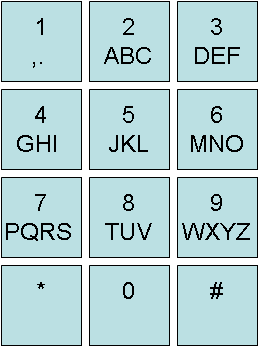
\includegraphics[scale=0.5]{img/itu-t.eps}
%%         \caption{an ITU-T keypad for mobile phone.}
%%         \label{fig:itut-keypad}
%%        \end{center}
%% \end{figure}

There are typical 2 methods to input an English word/phrase with ITU-T key pad.
For instance, if user wants to enter a word ``home'', He can press the key
in below sequence.

\begin{itemize}
\item Press key '4' twice to enter the letter 'h';
\item Press key '6' three times to enter the letter 'o';
\item Press key '6' twice to enter the letter 'm';
\item Press key '3' twice to enter the letter 'e';
\end{itemize}

Another high efficient way is to simplify the key press sequence like the
following.

\begin{itemize}
\item Press key '4', '6', '6', '3', word ``home'' appears on top of the candidate list;
\item Press key '*' to change a candidate word, so word ``good'' appears;
\item Press key '*' again to change another candidate word, next word ``gone'' appears;
\item ...
\end{itemize}

Compare these 2 method, we can see method 2 is much easier for the end user, and
it is operation efficient. The only overhead is to store a candidate words dictionary.

Method 2 is called as T9 input method, or predictive input method
\cite{wiki-t9}, \cite {wiki-predictive-text}. The abbreviation 'T9' stands
for 'textonym'. In this section, I'll show an example implementation of T9
by using Trie and Patricia.

In order to provide candidate words to user, a dictionary must be prepared
in advance. Trie or Patricia can be used to store the Dictionary. In the real
commercial software, complex indexing dictionary is used. We show the very 
simple Trie and Patricia only for illustration purpose.

\subsubsection{Iterative algorithm of T9 looking up}

Below pseudo code shows how to realize T9 with Trie.

\begin{algorithmic}
\STATE $TRIE-LOOK-UP-T9(T, key)$
  \STATE $PUSH-BACK(Q, NIL, key, T)$
  \STATE $r \leftarrow NIL$
  \WHILE{$Q$ is not empty}
    \STATE $p, k, t \leftarrow POP-FRONT(Q)$
    \STATE $i \leftarrow FIRST-LETTER(k)$
    \FOR{each $c$ in $T9-MAPPING(i)$}
      \IF{$c$ is in $CHILDREN(t)$}
        \STATE $k' \leftarrow k$ subtract $i$
        \IF{$k'$ is empty}
          \STATE $APPEND(r, p+c)$
        \ELSE
          \STATE $PUSH-BACK(Q, p+c, k', CHILDREN(t)[c])$
        \ENDIF
      \ENDIF
    \ENDFOR
  \ENDWHILE
  \RETURN $r$
\end{algorithmic}

This is actually a bread-first search program. It utilizes a queue to store
the current node and key string we are examining. The algorithm takes the first
digit from the key, looks up it in T9 mapping to get all English letters 
corresponding to this digit. For each letter, if it can be found in the children
of current node, the node along with the English string found so far are
push back to the queue. In case all digits are examined, a candidate is found.
We'll append this candidate to the result list. The loop will terminate when
the queue is empty.

Since Trie is not space effective, minor modification of the above program can
work with Patricia, which can help to save extra spaces.

\begin{algorithmic}
\STATE $PATRICIA-LOOK-UP-T9(T, key)$
  \STATE $PUSH-BACK(Q, NIL, key, T)$
  \STATE $r \leftarrow NIL$
  \WHILE{$Q$ is not empty}
    \STATE $p, k, t \leftarrow POP-FRONT(Q)$
    \FOR{each $child$ in $CHILDREN(t)$}
      \STATE $k' \leftarrow CONVERT-T9(KEY(child))$
      \IF{$k'$ IS-PREFIX-OF $k$}
        \IF{$k' = k$}
          \STATE $APPEND(r, p+KEY(child))$
        \ELSE
          \STATE $PUSH-BACK(Q, p+KEY(child), k-k', child)$
        \ENDIF
      \ENDIF
    \ENDFOR
  \ENDWHILE
  \RETURN $r$
\end{algorithmic}

\subsubsection*{T9 implementation in Python}

In Python implementation, T9 looking up is realized in a typical bread-first search algorithm as the following.

\lstset{language=Python}
\begin{lstlisting}
T9MAP={'2':"abc", '3':"def", '4':"ghi", '5':"jkl", \
       '6':"mno", '7':"pqrs", '8':"tuv", '9':"wxyz"}
                
def trie_lookup_t9(t, key):
    if t is None or key == "":
        return None
    q = [("", key, t)]
    res = []
    while len(q)>0:
        (prefix, k, t) = q.pop(0)
        i=k[0]
        if not i in T9MAP:
            return None #invalid input
        for c in T9MAP[i]:
            if c in t.children:
                if k[1:]=="":
                    res.append((prefix+c, t.children[c].value))
                else:
                    q.append((prefix+c, k[1:], t.children[c]))
    return res
\end{lstlisting}

Function trie\_lookup\_t9 check if the parameters are valid first. Then
it push the initial data into a queue. The program repeatedly pop the item
from the queue, including what node it will examine next, the number sequence
string, and the alphabetic string it has been searched.

For each popped item, the program takes the next digit from the number
sequence, and looks up in T9 map to find the corresponding English letters.
With all these letters, if they can be found in the children of the current
node, we'll push this child along with the updated number sequence string
and updated alphabetic string into the queue. In case we process all 
numbers, we find a candidate result.

We can verify the above program with the following test cases.

\begin{lstlisting}
class LookupTest:
    def __init__(self):
        t9dict = ["home", "good", "gone", "hood", "a", "another", "an"]
        self.t9t = trie.list_to_trie(t9dict)

    def test_trie_t9(self):
        print "search 4 ", trie_lookup_t9(self.t9t, "4")
        print "search 46 ", trie_lookup_t9(self.t9t, "46")
        print "search 4663 ", trie_lookup_t9(self.t9t, "4663")
        print "search 2 ", trie_lookup_t9(self.t9t, "2")
        print "search 22 ", trie_lookup_t9(self.t9t, "22")
\end{lstlisting}

If we run the test, it will output a very same result as the above Haskell
program.

\begin{verbatim}
search 4  [('g', None), ('h', None)]
search 46  [('go', None), ('ho', None)]
search 4663  [('gone', None), ('good', None), ('home', None), ('hood', None)]
search 2  [('a', None)]
search 22  []
\end{verbatim}

To save the spaces, Patricia can be used instead of Trie.

\begin{lstlisting}
def patricia_lookup_t9(t, key):
    if t is None or key == "":
        return None
    q = [("", key, t)]
    res = []
    while len(q)>0:
        (prefix, key, t) = q.pop(0)
        for k, tr in t.children.items():
            digits = toT9(k)
            if string.find(key, digits)==0: #is prefix of
                if key == digits:
                    res.append((prefix+k, tr.value))
                else:
                    q.append((prefix+k, key[len(k):], tr))
    return res
\end{lstlisting}

Compare to the implementation with Trie, they are very similar. We also 
used a bread-first search approach. The different part is that we convert
the string of each child to number sequence string according to T9 mapping.
if it is prefix of the key we are looking for, we push this child along with
updated key and prefix. In case we examined all digits, we find a candidate
result.

The convert function is a reverse mapping process as below.
\begin{lstlisting}
def toT9(s):
    res=""
    for c in s:
        for k, v in T9MAP.items():
            if string.find(v, c)>=0:
                res+=k
                break
        #error handling skipped.
    return res
\end{lstlisting}

For illustration purpose, the error handling for invalid letters is skipped.
If we feed the program with the same test cases, we can get a result as the 
following.

\begin{verbatim}
search 4  []
search 46  [('go', None), ('ho', None)]
search 466  []
search 4663  [('good', None), ('gone', None), ('home', None), ('hood', None)]
search 2  [('a', None)]
search 22  []
\end{verbatim}

The result is slightly different from the one output by Trie. The reason is
as same as what we analyzed in Haskell implementation. It is easily to modify
the program to output a similar result.

\subsubsection*{T9 implemented in C++}

First we define T9 mapping as a Singleton object, this is because we
want to it can be used both in Trie look up and Patricia look up programs.

\lstset{language=C++}
\begin{lstlisting}
struct t9map{
  typedef std::map<char, std::string> Map;
  Map map;

  t9map(){
    map['2']="abc";
    map['3']="def";
    map['4']="ghi";
    map['5']="jkl";
    map['6']="mno";
    map['7']="pqrs";
    map['8']="tuv";
    map['9']="wxyz";
  }

  static t9map& inst(){
    static t9map i;
    return i;
  }
};
\end{lstlisting}

Note in other languages or keypad layout, we can define different
mappings and pass them as a parameter to the looking up function.

With this mapping, the looking up in Trie can be given as
below. Although we want to keep the genericity of the program, for
illustration purpose, we just simply use the t9 mapping directly.

In order to keep the code as short as possible, a boost library tool,
boost::tuple is used. For more about boost::tuple, please refer to \cite{boost-book}.

\begin{lstlisting}
template<class K, class V>
std::list<std::pair<K, V> > lookup_t9(Trie<K, V>* t,
				      typename Trie<K, V>::KeyType key)
{
  typedef std::list<std::pair<K, V> > Result;
  typedef typename Trie<K, V>::KeyType Key;
  typedef typename Trie<K, V>::Char Char;

  if((!t) || key.empty())
    return Result();
  
  Key prefix;
  std::map<Char, Key> m = t9map::inst().map;
  std::queue<boost::tuple<Key, Key, Trie<K, V>*> > q;
  q.push(boost::make_tuple(prefix, key, t));
  Result res;
  while(!q.empty()){
    boost::tie(prefix, key, t) = q.front();
    q.pop();
    Char c = *key.begin();
    key = Key(key.begin()+1, key.end());
    if(m.find(c) == m.end())
      return Result();
    Key cs = m[c];
    for(typename Key::iterator it=cs.begin(); it!=cs.end(); ++it)
      if(t->children.find(*it)!=t->children.end()){
	if(key.empty())
	  res.push_back(std::make_pair(prefix+*it, t->children[*it]->value));
	else
	  q.push(boost::make_tuple(prefix+*it, key, t->children[*it]));
      }
  }
  return res;
}
\end{lstlisting}

This program will first check if the Patricia tree or the key are
empty to deal with with trivial case. It next initialize a queue, and
push one tuple to it. the tuple contains 3 elements, a prefix to
represent a string the program has been searched, current key it need
look up, and a node it will examine. 

Then the program repeatedly pops the tuple from the queue, takes the
first character from the key, and looks up in T9 map to get a
candidate English letter list. With each letter in this list, the
program examine if it exists in the children of current node. In case
it find such a child, if there is no left letter to look up, it means
we found a candidate result, we push it to the result list. Else, we
create a new tuple with updated prefix, key and this child; the push
it to the queue for later process.

Below are some simple test cases for verification.

\begin{lstlisting}
Trie<std::string, std::string>* t9trie(0);
const char* t9dict[] = {"home", "good", "gone", "hood", "a", "another", "an"};
t9trie = list_to_trie(t9dict, t9dict+sizeof(t9dict)/sizeof(char*), t9trie);
std::cout<<"test t9 lookup in Trie\n"
         <<"search 4 "<<lop_to_str(lookup_t9(t9trie, "4"))<<"\n"
	 <<"serach 46 "<<lop_to_str(lookup_t9(t9trie, "46"))<<"\n"
	 <<"serach 4663 "<<lop_to_str(lookup_t9(t9trie, "4663"))<<"\n"
	 <<"serach 2 "<<lop_to_str(lookup_t9(t9trie, "2"))<<"\n"
	 <<"serach 22 "<<lop_to_str(lookup_t9(t9trie, "22"))<<"\n\n";
delete t9trie;
\end{lstlisting}

It will output the same result as the Python program.

\begin{verbatim}
test t9 lookup in Trie
search 4 [(g, ), (h, ), ]
serach 46 [(go, ), (ho, ), ]
serach 4663 [(gone, ), (good, ), (home, ), (hood, ), ]
serach 2 [(a, ), ]
serach 22 []
\end{verbatim}

In order to save space, a looking up program for Patricia is also
provided.

\begin{lstlisting}
template<class K, class V>
std::list<std::pair<K, V> > lookup_t9(Patricia<K, V>* t,
				      typename Patricia<K, V>::KeyType key)
{
  typedef std::list<std::pair<K, V> > Result;
  typedef typename Patricia<K, V>::KeyType Key;
  typedef typename Key::value_type Char;
  typedef typename Patricia<K, V>::Children::iterator Iterator;

  if((!t) || key.empty())
    return Result();

  Key prefix;
  std::map<Char, Key> m = t9map::inst().map;
  std::queue<boost::tuple<Key, Key, Patricia<K, V>*> > q;
  q.push(boost::make_tuple(prefix, key, t));
  Result res;
  while(!q.empty()){
    boost::tie(prefix, key, t) = q.front();
    q.pop();
    for(Iterator it=t->children.begin(); it!=t->children.end(); ++it){
      Key digits = t9map::inst().toT9(it->first);
      if(is_prefix_of(digits, key)){
	if(digits == key)
	  res.push_back(std::make_pair(prefix+it->first, it->second->value));
	else{
	  key =Key(key.begin()+it->first.size(), key.end());
	  q.push(boost::make_tuple(prefix+it->first, key, it->second));
	}
      }
    }
  }
  return res;
}
\end{lstlisting}

The program is similar to the one with Trie very much. This is a
typical bread-first search approach. Note that we added a member
function to\_t9() to convert a English word/phrase back to digit
number string. This member function is implemented as the following.

\begin{lstlisting}
struct t9map{
  //...
  std::string to_t9(std::string s){
    std::string res;
    for(std::string::iterator c=s.begin(); c!=s.end(); ++c){
      for(Map::iterator m=map.begin(); m!=map.end(); ++m){
	std::string val = m->second;
	if(std::find(val.begin(), val.end(), *c)!=val.end()){
	  res.push_back(m->first);
	  break;
	}
      }
    } // skip error handling.
    return res;
  }
\end{lstlisting}

The error handling for invalid letters is omitted in order to keep the
code short for easy understanding. We can use the very similar test
cases as above except we need change the Trie to Patrica. It will
output as below.

\begin{verbatim}
test t9 lookup in Patricia
search 4 []
serach 46 [(go, ), (ho, ), ]
serach 466 []
serach 4663 [(gone, ), (good, ), ]
serach 2 [(a, ), ]
serach 22 []
\end{verbatim}

The result is slightly different, please refer to the Haskell section
for the reason of this difference. It is very easy to modify the
program to output the very same result as Trie's one.

\subsubsection{Recursive algorithm of T9 looking up}

\subsubsection*{T9 implemented in Haskell}

In Haskell, we first define a map from key pad to English letter. When user
input a key pad number sequence, we take each number and check from the Trie.
All children match the number should be investigated. Below is a Haskell 
program to realize T9 input.

\lstset{language=Haskell}
\begin{lstlisting}
mapT9 = [('2', "abc"), ('3', "def"), ('4', "ghi"), ('5', "jkl"), 
         ('6', "mno"), ('7', "pqrs"), ('8', "tuv"), ('9', "wxyz")]

lookupT9 :: Char -> [(Char, b)] -> [(Char, b)]
lookupT9 c children = case lookup c mapT9 of
        Nothing -> []
        Just s  -> foldl f [] s where
             f lst x = case lookup x children of
                 Nothing -> lst
                 Just t  -> (x, t):lst
        
-- T9-find in Trie
findT9:: Trie a -> String -> [(String, Maybe a)]
findT9 t [] = [("", Trie.value t)]
findT9 t (k:ks) = foldl f [] (lookupT9 k (children t))
    where
      f lst (c, tr) = (mapAppend c (findT9 tr ks)) ++ lst
\end{lstlisting}

findT9 is the main function, it takes 2 parameters, a Trie and a number
sequence string. In non-trivial case, it calls lookupT9 function to
examine all children which match the first number.

For each matched child, the program recursively calls findT9 on it with
the left numbers, and we use mapAppend to insert the currently finding letter
in front of all results. The program use foldl to combine all these together.

Function lookupT9 is used to filtered all possible children who match a
number. It first call lookup function on mapT9, so that a string of possible
English letters can be identified. Next we call lookup for each candidate
letter to see if there is a child can match the letter. We use foldl to 
collect all such child together.

This program can be verified by using some simple test cases.

\begin{lstlisting}
testFindT9 = "press 4: " ++ (show $ take 5 $ findT9 t "4")++
             "\npress 46: " ++ (show $ take 5 $ findT9 t "46")++
             "\npress 4663: " ++ (show $ take 5 $ findT9 t "4663")++
             "\npress 2: " ++ (show $ take 5 $ findT9 t "2")++
             "\npress 22: " ++ (show $ take 5 $ findT9 t "22")
    where
      t = Trie.fromList lst
      lst = [("home", 1), ("good", 2), ("gone", 3), ("hood", 4), 
             ("a", 5), ("another", 6), ("an", 7)]
\end{lstlisting}

The program will output below result.

\begin{verbatim}
press 4: [("g",Nothing),("h",Nothing)]
press 46: [("go",Nothing),("ho",Nothing)]
press 4663: [("gone",Just 3),("good",Just 2),("home",Just 1),("hood",Just 4)]
press 2: [("a",Just 5)]
press 22: []
\end{verbatim}

The value of each child is just for illustration, we can put empty value instead
and only returns candidate keys for a real input application.

Tries consumes to many spaces, we can provide a Patricia version as alternative.

\begin{lstlisting}
findPrefixT9' :: String -> [(String, b)] -> [(String, b)]
findPrefixT9' s lst = filter f lst where
    f (k, _) = (toT9 k) `Data.List.isPrefixOf` s

toT9 :: String -> String
toT9 [] = []
toT9 (x:xs) = (unmapT9 x mapT9):(toT9 xs) where
    unmapT9 x (p:ps) = if x `elem` (snd p) then (fst p) else unmapT9 x ps

findT9' :: Patricia a -> String -> [(String, Maybe a)]
findT9' t [] = [("", value t)]
findT9' t k = foldl f [] (findPrefixT9' k (children t)) 
    where
      f lst (s, tr) = (mapAppend' s (findT9' tr (k `diff` s))) ++ lst
      diff x y = drop (length y) x
\end{lstlisting}

In this program, we don't check one digit at a time, we take all the digit
sequence, and we examine all children of the Patricia node. For each child,
the program convert the prefix string to number sequence by using function 
toT9, if the result is prefix of what user input, we go on search in this 
child and append the prefix in front of all further results.

If we tries the same test case, we can find the result is a bit different.

\begin{verbatim}
press 4: []
press 46: [("go",Nothing),("ho",Nothing)]
press 466: []
press 4663: [("good",Just 2),("gone",Just 3),("home",Just 1),("hood",Just 4)]
press 2: [("a",Just 5)]
press 22: []
\end{verbatim}

If user press key '4', because the dictionary (represent by Patricia) doesn't
contain any candidates matches it, user will get an empty candidates list.
The same situation happens when he enters ``466''. In real input method 
implementation, such user experience isn't good, because it displays nothing
although user presses the key several times. One improvement is to 
predict what user will input next by display a partial result. This can be 
easily achieved by modify the above program. (Hint: not only check
\begin{lstlisting}
findPrefixT9' s lst = filter f lst where
    f (k, _) = (toT9 k) `Data.List.isPrefixOf` s
\end{lstlisting}
but also check
\begin{lstlisting}
    f (k, _) = s `Data.List.isPrefixOf` (toT9 k)
\end{lstlisting}
)

\subsubsection*{T9 implemented in Scheme/Lisp}

In Scheme/Lisp, T9 map is defined as a list of pairs.

\lstset{language=lisp}
\begin{lstlisting}
(define map-T9 (list '("2" "abc") '("3" "def") '("4" "ghi") '("5" "jkl")
		     '("6" "mno") '("7" "pqrs") '("8" "tuv") '("9" "wxyz")))
\end{lstlisting}

The main searching function is implemented as the following.

\begin{lstlisting}
(define (find-T9 t k) ;; return [(key value)]
  (define (accumulate-find lst child)
    (append (map-string-append (key child) (find-T9 (tree child) (string-cdr k))) 
	    lst))
  (define (lookup-child lst c) ;; lst, list of childen [(key tree)], c, char
    (let ((res (find-matching-item map-T9 (lambda (x) (string=? c (car x))))))
      (if (not res) '()
	  (filter (lambda (x) (substring? (key x) (cadr res))) lst))))
  (if (string-null? k) (list (cons k (value t)))
      (fold-left accumulate-find '() (lookup-child (children t) (string-car k)))))
\end{lstlisting}

This function contains 2 inner functions. If the string is empty, the
program returns a one element list. The element is a string value pair.
For the none trivial case, the program will call inner function to
find in each child and then put them together by using fold-left high
order function.

To test this T9 search function, a very simple dictionary is
established by using Trie insertion. Then we test by calling find-T9
function on several digits sequences.

\begin{lstlisting}
(define dict-T9 (list '("home" ()) '("good" ()) '("gone" ()) '("hood" ()) 
		      '("a" ()) '("another" ()) '("an" ())))

(define (test-trie-T9)
  (define t (list->trie dict-T9))
  (display "find 4: ") (display (find-T9 t "4")) (newline)
  (display "find 46: ") (display (find-T9 t "46")) (newline)
  (display "find 4663: ") (display (find-T9 t "4663")) (newline)
  (display "find 2: ") (display (find-T9 t "2")) (newline)
  (display "find 22: ") (display (find-T9 t "22")) (newline))
\end{lstlisting}

Evaluate this test function will output below result.

\begin{verbatim}
find 4: ((g) (h))
find 46: ((go) (ho))
find 4663: ((gone) (good) (hood) (home))
find 2: ((a))
find 22: ()
\end{verbatim}

In order to be more space effective, Patricia can be used to replace
Trie. The search program modified as the following.

\begin{lstlisting}
(define (find-T9 t k)
  (define (accumulate-find lst child)
    (append (map-string-append (key child) (find-T9 (tree child) (string- k (key child))))
	    lst))
  (define (lookup-child lst k)
    (filter (lambda (child) (string-prefix? (str->t9 (key child)) k)) lst))
  (if (string-null? k) (list (cons "" (value t)))
      (fold-left accumulate-find '() (lookup-child (children t) k))))
\end{lstlisting}

In this program a string helper function 'string-' is defined to get
the different part of two strings. It is defined like below.

\begin{lstlisting}
(define (string- x y)
  (string-tail x (string-length y)))
\end{lstlisting}

Another function is 'str->t9' it will convert a alphabetic string back
to digit sequence base on T9 mapping.

\begin{lstlisting}
(define (str->t9 s)
  (define (unmap-t9 c)
    (car (find-matching-item map-T9 (lambda (x) (substring? c (cadr x))))))
  (if (string-null? s) ""
      (string-append (unmap-t9 (string-car s)) (str->t9 (string-cdr s)))))
\end{lstlisting}

We can feed the almost same test cases, and the result is output as
the following.

\begin{verbatim}
find 4: ()
find 46: ((go) (ho))
find 466: ()
find 4663: ((good) (gone) (home) (hood))
find 2: ((a))
find 22: ()
\end{verbatim}

Note the result is a bit different, the reason is described in Haskell
section. It is easy to modify the program, so that Trie and Patricia
approach give the very same result.

% ================================================================
%                 Short summary
% ================================================================
\section{Notes and short summary}

Suffix Tree was first introduced by Weiner in 1973 \cite{weiner}.

In this post, we start from the Integer base trie and Patricia, the
map data structure based on integer patricia plays an important role
in Compiler implementation. Next, alphabetic Trie and Patricia are
given, and I provide a example implementation to illustrate how to
realize a predictive e-dictionary and a T9 input method. Although they
are far from the real implementation in commercial software. They show
a very simple approach of manipulating text. There are still some
interesting problem can not be solved by Trie or Patrica directly, how
ever, some other data structures such as suffix tree have close
relationship with them. I'll note something about suffix tree in other post.

% ================================================================
%                 Appendix
% ================================================================
\section{Appendix} \label{appendix}
%\appendix
All programs provided along with this article are free for
downloading.

\subsection{Prerequisite software}
GNU Make is used for easy build some of the program. For C++ and ANSI C programs,
GNU GCC and G++ 3.4.4 are used. I use boost triple to reduce the
amount of our code lines, boost library version I am using is
1.33.1. The path is in CXX variable in Makefile, please change it to
your path when compiling.
For Haskell programs GHC 6.10.4 is used
for building. For Python programs, Python 2.5 is used for testing, for
Scheme/Lisp program, MIT Scheme 14.9 is used.

all source files are put in one folder. Invoke 'make' or 'make all'
will build C++ and Haskell program. 

Run 'make Haskell' will separate build Haskell program. There will be
two executable file generated one is htest the other is happ (with .exe
in Window like OS). Run htest will test functions in IntTrie.hs, IntPatricia.hs,
Trie.hs and Patricia.hs. Run happ will execute the editionary and T9
test cases in EDict.hs.

Run 'make cpp' will build c++ program. It will create a executable
file named cpptest (with .exe in Windows like OS). Run this program
will test inttrie.hpp, intpatricia.hpp, trie.hpp, patricia.hpp, and
edict.hpp. 

Run 'make c' will build the ANSI C program for Trie. It will create a
executable file named triec (with .exe in Windows like OS).

Python programs can run directly with interpreter. 

Scheme/Lisp program need be loaded into Scheme evaluator and evaluate
the final function in the program. Note that patricia.scm will hide
some functions defined in trie.scm.

Here is a detailed list of source files

\subsection{Haskell source files}

\begin{itemize}
\item IntTrie.hs, Haskell version of little-endian integer Trie.
\item IntPatricia.hs, integer Patricia tree implemented in Haskell.
\item Trie.hs, Alphabetic Trie, implemented in Haskell.
\item Patricia.hs, Alphabetic Patricia, implemented in Haskell.
\item TestMain.hs, main module to test the above 4 programs.
\item EDict.hs, Haskell program for e-dictionary and T9.
\end{itemize}

\subsection{C++/C source files}

\begin{itemize}
\item inttrie.hpp, Integer base Trie;
\item intpatricia.hpp, Integer based Patricia tree;
\item trie.c, Alphabetic Trie only for lowercase English language,
implemented in ANSI C. 
\item trie.hpp, Alphabetic Trie;
\item patricia.hpp, Alphabetic Patricia;
\item trieutil.hpp, Some generic utilities;
\item edit.hpp, e-dictionary and T9 implemented in C++;
\item test.cpp, main program to test all above programs.
\end{itemize}

\subsection{Python source files}

\begin{itemize}
\item inttrie.py, Python version of little-endian integer Trie, with
test cases;
\item intpatricia.py, integer Patricia tree implemented in Python;
\item trie.py, Alphabetic Trie, implemented in Python;
\item patricia.py, Alphabetic Patricia implemented in Python;
\item trieutil.py, Common utilities;
\item edict.py, e-dictionary and T9 implemented in Python.
\end{itemize}

\subsection{Scheme/Lisp source files}

\begin{itemize}
\item inttrie.scm, Little-endian integer Trie, implemented in Scheme/Lisp;
\item intpatricia.scm, Integer based Patricia tree;
\item trie.scm, Alphabetic Trie;
\item patricia.scm, Alphabetic Patricia, reused many definitions in
Trie;
\item trieutil.scm, common functions and utilities.
\end{itemize}

\subsection{Tools}

Besides them, I use graphviz to draw most of the figures in this post. In order to
translate the Trie, Patrica and Suffix Tree output to dot language scripts. I wrote a python program.
it can be used like this.

\begin{verbatim}
trie2dot.py -o foo.dot -t patricia "1:x, 4:y, 5:z"
trie2dot.py -o foo.dot -t trie "001:one, 101:five, 100:four"
\end{verbatim}

This helper scripts can also be downloaded with this article.

download position: http://sites.google.com/site/algoxy/trie/trie.zip

\begin{thebibliography}{99}

\bibitem{ukkonen95}
Esko Ukkonen. ``On-line construction of suffix trees''. Algorithmica 14 (3): 249--260. doi:10.1007/BF01206331. http://www.cs.helsinki.fi/u/ukkonen/SuffixT1withFigs.pdf

\bibitem{wiki-suffix-tree}
Suffix Tree, Wikipedia. http://en.wikipedia.org/wiki/Suffix\_tree

\bibitem{ukkonen-presentation}
Esko Ukkonen. ``Suffix tree and suffix array techniques for pattern ananlysis in strings''. http://www.cs.helsinki.fi/u/ukkonen/Erice2005.ppt

\bibitem{wiki-trie}
Trie, Wikipedia. http://en.wikipedia.org/wiki/Trie

\bibitem{lxy-trie}
Liu Xinyu. ``Trie and Patricia, with Functional and imperative implementation''. http://sites.google.com/site/algoxy/trie

\end{thebibliography}

\ifx\wholebook\relax\else
\end{document}
\fi
